\chapter{\textbf{Conception et mise en oeuvre du système MoPlaZer}}
    \section{Introduction}
    En nous basant des travaux des chercheurs dans le domaine informatique, nous avons fait dans les chapitres précédents des études théoriques des axes principaux de notre sujet sur les systèmes ANPR. Ces études nous ont permis de concevoir et mettre en place aussi notre système de reconnaissance automatique des plaques d'immatriculation. Ce chapitre est donc pour mettre en lumière ce système. Pour cela, nous commencerons par présenter l'architecture simple que nous avons opté pour. Par la suite, nous détaillerons chaque partie de cette architecture. Il est bien de préciser que nous parlons ici de l'architecture logicielle de notre système et non pas du côté matériel.
    
    \section{Architecture}
Le système ANPR que nous avons réalisé est essentiellement composé de deux grandes parties:
    \begin{enumerate}
        \item \textbf{Une partie de détection de la plaque}: Dans cette partie, on veut répondre à la question suivante: où se trouve la plaque sur l'image ? En effet, avant de reconnaître le numéro d'immatriculation, il est important de localiser premièrement la position de la plaque sur l'image reçue à travers la caméra. À partir de cette localisation, on peut isoler la plaque du reste de l'image pour l'envoyer à la partie suivante.
        \item \textbf{Une partie de lecture des caractères}: L'entrée de cette partie est la sortie de la partie précédente. L'objectif de cette partie est de reconnaître l'ensemble des caractères sur l'image de la plaque. Cette partie du système retourne alors le numéro du matricule présent sur l'image en format textuel ou ASCII enregistrable dans une base de données.
    \end{enumerate}
    La figure suivante illustre l'architecture que nous avons choisie pour notre système ANPR.
    \begin{figure}[H]
        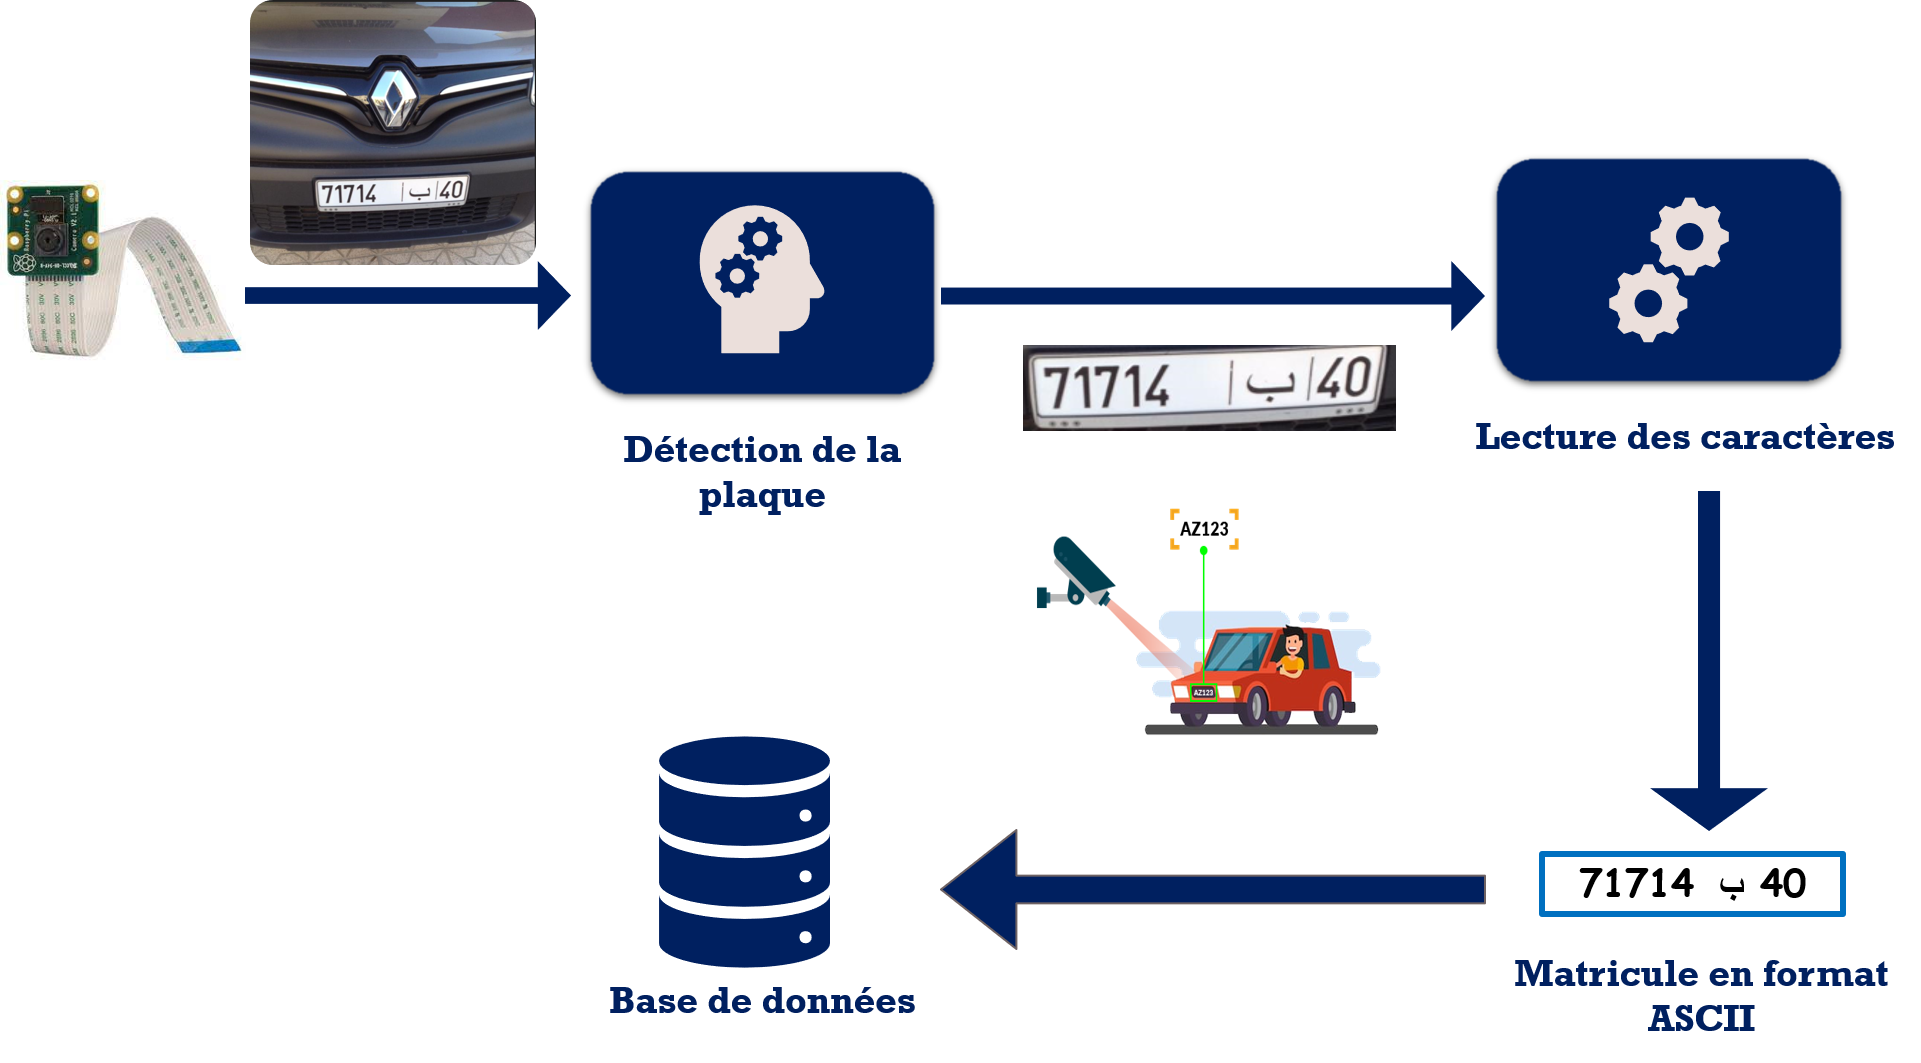
\includegraphics[scale=0.5]{moplazer}
        \caption{Architecture du système MoPlaZer}
    \end{figure}
    \section{Détection de la plaque}
Pour détecter la plaque sur une image, nous avons choisi l’approche par apprentissage automatique. À cet effet, nous avons entraîné un modèle Deep Learning de détection d’objets en utilisant l’architecture YOLOv4 Tiny. Le choix de cette architecture s’explique par ses performances qui sont clairement définies dans le tableau \ref{table:yolo}. D’autre part, cette architecture est la plus adaptée pour les appareils mobiles et systèmes embarqués où nous allons déployer le modèle de détection. Décrivons maintenant chaque étape que nous avons suivie pour avoir le modèle.
    \subsection{Acquisition des données}
    L’entraînement d’un modèle de Deep Learning nécessite une masse importante de données. Pour le détection des plaques, nous avons collecté les images de véhicules sur la plateforme \textbf{Open Images de Google}. Open Images est un ensemble de données d'environ 9 millions d'images annotées avec des étiquettes au niveau des images, des cadres de délimitation d'objets, des masques de segmentation d'objets, des relations visuelles et des récits localisés \cite{oid6}. Sur cette plateforme, nous avons pu  avoir \textbf{5890 images avec les annotations sous format YOLO d’une taille d’environ 2Go}. Les annotations sont des fichiers texte contenant les coordonnées des cadres de délimitation des plaques. 
    \begin{figure}[H]
        \centering
        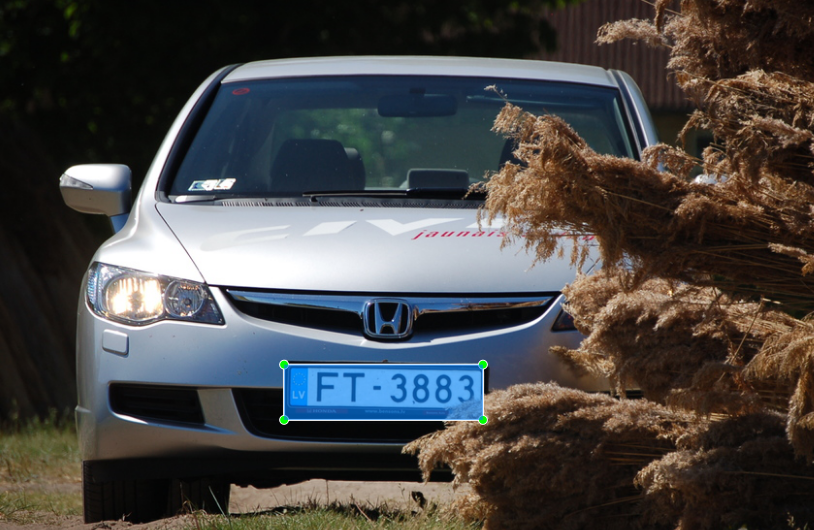
\includegraphics[scale=0.3]{imageDataset}
        \caption{Exemple d'images collectées sur Open Images}
    \end{figure}
    Après une analyse des données collectées, voici quelques unes de ses caractéristiques:
    \begin{table}[H]
        \centering
        \begin{tabular}{|l|l|}
            \hline
            \rowcolor{Gray}
            \textbf{Caractéristiques} & \textbf{Valeur} \\ \hline
            Largeur maximale des images & \textbf{2672px} \\ \hline
            Hauteur maximale des images & \textbf{4000px} \\ \hline
            Largeur minimale des images & \textbf{141px} \\ \hline
            Hauteur minimale des images & \textbf{225px} \\ \hline
            Nombre maximal d'annotations sur une image & \textbf{26} \\ \hline
            Moyenne du nombre d'annotations par image & \textbf{1.43} \\ \hline
            Nombres d'images dupliquées & \textbf{134} \\ \hline
        \end{tabular}
        \caption{Analyse de la collection des données de véhicules}
    \end{table}
    \subsection{Nettoyage et préparation}
    Avant d’utiliser les données collectées, il est important de les vérifier et corriger les anomalies afin d’éviter des mauvaises performances du modèle. A l’aide de l’outil d’annotations \textbf{LabelImg}, nous avons vérifié si toutes les images que nous avions chargées étaient bien annotées. Dans certains cas rares, il fallait recadrer le rectangle délimitant la plaque d’immatriculation. D’autre part, nous avons remarqué comme l’indique le tableau précédent que 134 images ont été dupliquées. A l’aide d’un script écrit en Python, nous avons supprimé toutes ces duplications. Nous obtenons finalement une base de données de 5756 images distinctes et correctement annotées. Par ailleurs, grâce à la plateforme en ligne Roboflow, nous avons effectué quelques opérations de prétraitement sur l’ensemble des images. Ces opérations permettent d’une part de réduire le temps d’entraînement du modèle et d’autre part d'améliorer la précision du modèle. Parmi ces opérations, on retrouve l’\textbf{auto-orientation} pour standardiser l’ordre des pixels et le \textbf{redimensionnement à 416 x 416} (taille d’entrée du modèle).
    \subsection{Entraînement du modèle}
    Pour l’évaluation de la performance du modèle au cours de l’entraînement, nous avons subdivisé notre base de données en deux grands groupes: 80\% soit 4604 images pour l’entraînement et 20\% pour le test. L’entraînement du modèle a été fait sur la plateforme en ligne Google Colab. Elle offre des ressources(puissance de GPU) gratuitement pour entraîner des modèles de Deep Learning. Voici quelques configurations prises en compte:
    \begin{itemize}
        \item \textbf{Type d'exécution: GPU}
        \item \textbf{Utilisation de CUDA Version 11.2}
        \item \textbf{GPU: Tesla T4}
        \item \textbf{Architecture du modèle: YOLO V4}
        \item \textbf{Utilisation de Tensorflow version 2.3.0rc0}
        \item \textbf{Utilisation du \href{https://github.com/roboflow-ai/darknet.git}{repertoire darknet de Roboflow}}
        \item \textbf{Utilisation de fichier de configuration} \href{https://github.com/AlexeyAB/darknet/blob/master/cfg/yolov4-tiny-3l.cfg}{yolov4-tiny\_3l.cfg}: Toutefois nous avons modifié certains paramètres dans ce fichier.
        \begin{table}[H]
            \centering
            \begin{tabular}{|l|c|}
                \hline
                \rowcolor{Gray}
                \textbf{Paramètres} & \textbf{Nouvelle valeur} \\ \hline
                batch & 64 \\ \hline
                subdivisions & 32 \\ \hline
                width & 416 \\ \hline
                height & 416 \\ \hline
                max\_batches & 6000 \\ \hline
                steps & 4800, 5400 \\ \hline
                classes & 1 \\ \hline
                filters (couche de convolution avant couche yolo) & 18 \\ \hline 
            \end{tabular}
            \caption{Quelques paramètres du fichier de configuration YOLO}
        \end{table}
        \item \textbf{Utilisation des poids pré-entraînés YOLO: \href{https://github.com/AlexeyAB/darknet/releases/download/darknet_yolo_v4_pre/yolov4-tiny.conv.29}{yolov4-tiny.conv.29}} 
    \end{itemize}
    L’entraînement a pratiquement pris 1.5 heures. Voici une courbe montrant l’évolution de la précision du modèle au cours de l’entraînement:
    \begin{figure}[H]
        \centering
        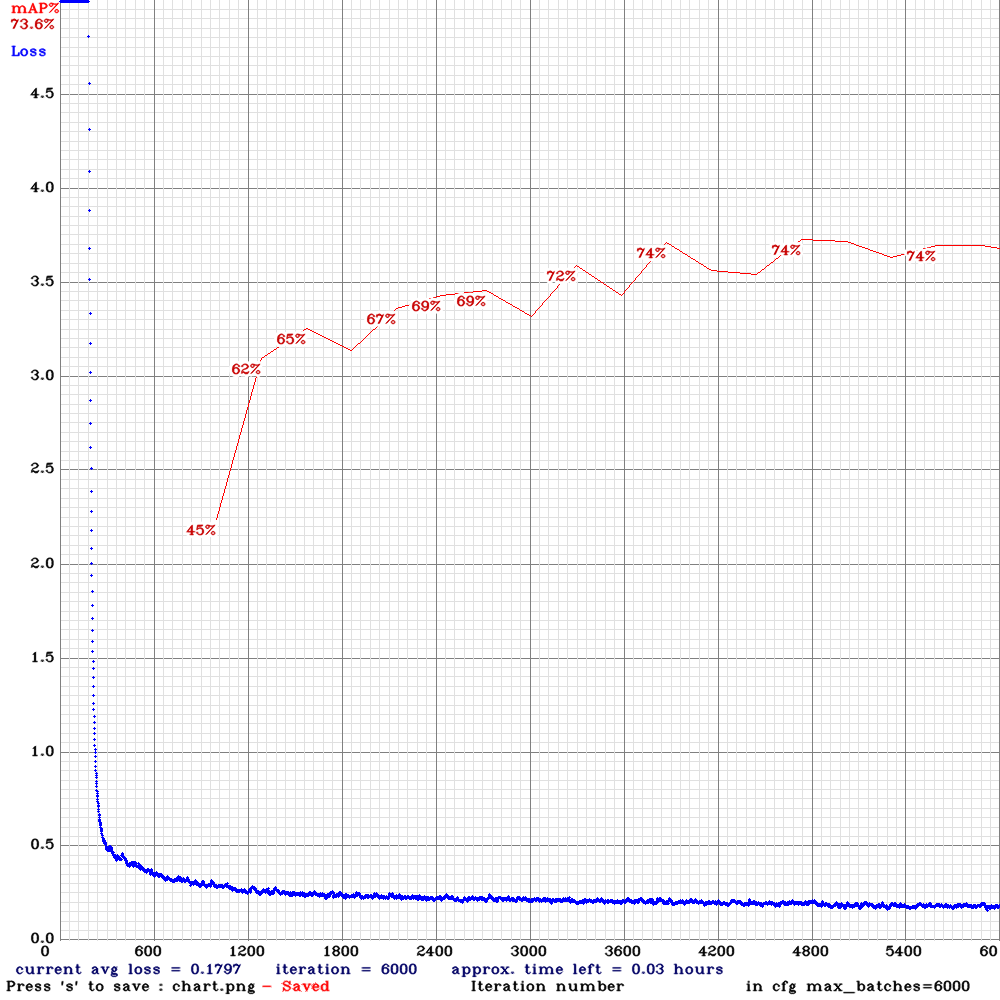
\includegraphics[scale=0.3]{chart1.png}
        \caption{Évolution de la métrique mAP lors de l'entraînement du modèle de détection de plaques.}
    \end{figure}
    À la fin de l'entraînement, le modèle est un fichier binaire extension \textbf{.weights}. Ce fichier contient les poids du réseaux de neurones. Par ailleurs, nous constatons à partir de la courbe précédente que la précision maximale qu'atteint le modèle au cours de son entraînement est de \textbf{74\%}.
    \subsection{Résultats et évaluation}
    Nous avons évalué notre modèle de détection des plaques sur deux types de données: les images contenant des véhicules au Maroc pour évaluer la précision du modèle et les vidéos de voitures en circulation pour mesurer la rapidité du modèle. 
    
    
    Pour le premier type, nous avons collecté des images sur les plateformes comme Kaggle, MSDA Datasets de UM6P et d’autres prises dans la rue. Après avoir réuni ces différentes sources de données, nous avons obtenu une base de données de 2229 images. On retrouve en moyenne une plaque par image. Le tableau d’évaluation est décrit comme suit:
    \begin{table}[H]
        \centering
        \begin{tabular}{|l|l|}
            \hline
            \rowcolor{Gray}
            \textbf{Evaluation} & \textbf{Valeur} \\ \hline
            Nombre de plaques correctement détectées (VP) & \textbf{1994} \\ \hline
            Nombre de plaques non détectées (FN) & \textbf{386} \\ \hline
            Nombre de fausses détections (FP) & \textbf{6} \\ \hline
            Précision & \textbf{99,7\%} \\ \hline
            Rappel & \textbf{83,78\%} \\ \hline
        \end{tabular}
        \caption{Evaluation du modèle de détection des plaques marocaines}
    \end{table}
    Puisque la précision et le rappel du modèle sont élevés, on peut dire que le modèle est performant en terme de précision de détection. La figure suivante traduit des exemples de détection faite par le modèle qui a été entraîné.
    \begin{figure}[H]
        \begin{subfigure}{0.3\textwidth}
            \centering
            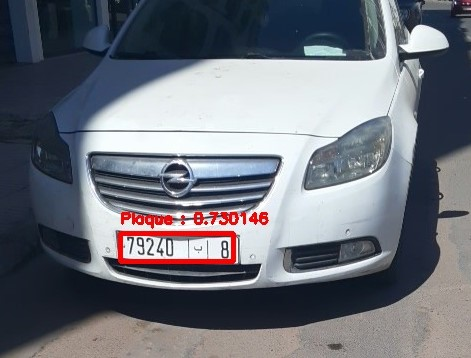
\includegraphics[width=\textwidth]{carMorocco232.jpg}
        \end{subfigure}
        \hfill
        \begin{subfigure}{0.3\textwidth}
            \centering
            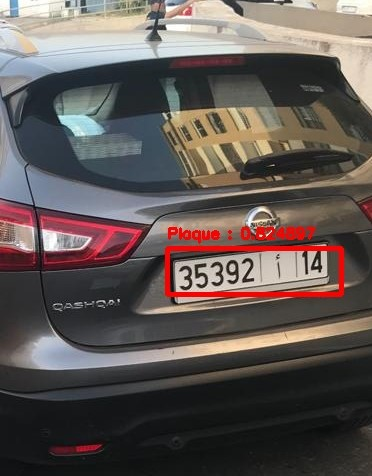
\includegraphics[width=\textwidth]{carMorocco772.jpg}
        \end{subfigure}
        \hfill
        \begin{subfigure}{0.3\textwidth}
            \centering
            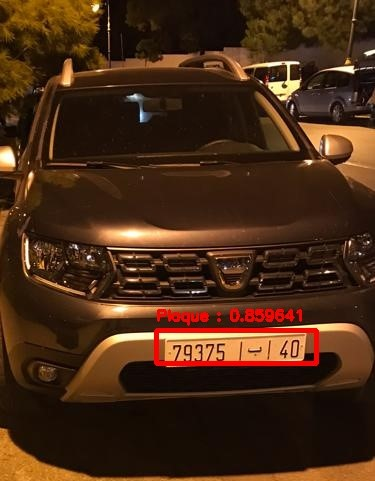
\includegraphics[width=\textwidth]{carMorocco913.jpg}
        \end{subfigure}
        \caption{Exemples de détection de plaques marocaines}
    \end{figure}
    Pour évaluer la rapidité de notre modèle, nous avons lancé le modèle sur des vidéos des véhicules en circulation. Puisque cette rapidité dépend à partie des performances matérielles de la machine sur laquelle le modèle est exécuté, voici ces caractéristiques:
    \begin{table}[H]
        \centering
        \begin{tabular}{|l|l|}
            \hline
            \rowcolor{Gray}
            \textbf{Caractèristiques} & \textbf{Valeur} \\ \hline
            Processeur & \textbf{Intel(R) Core(TM) i5-10210U CPU @ 1.60GHz   2.11 GHz} \\ \hline
            RAM & \textbf{8.00 Go} \\ \hline
            Disque dur SSD & \textbf{237 Go} \\ \hline
            Type de système & \textbf{Système d’exploitation 64 bits, processeur x64} \\ \hline
        \end{tabular}
        \caption{Caractèristiques du PC}
    \end{table}
    Avec un script Python en utilisant la librairie de traitement d’images OpenCV, nous avons constaté qu’avec les performances ci-dessus, notre modèle traite environ \textbf{14 à 18 images par secondes} en d’autres termes \textbf{14-18 FPS}.
    
    \section{Lecture du numéro d'immatriculation}
Pour la lecture des caractères présents sur la plaque détectée, nous avons utilisé une approche proposée par certains chercheurs de l’UM6P \cite{Alahyane2021OpenDF}. Cette approche consiste à utiliser un modèl de Deep Learning pour détecter les caractères et classifier en même temps. Pour l’entraînement du modèle, ils ont fait appel à l’architecture YOLOv3. La précision obtenue sur les données d’entraînement était de \textbf{94,42\%} et sur les données de test \textbf{82,38\%}. Puisque ces résultats sont satistfaisants, nous avons adopté la même approche mais avec une version plus récente de YOLO: version 4. L'avantage avec cette approche par l'approche classique de l'OCR est que nous n'avons pas vraiment besoin d'une phase de prétraitement de l'image au préalable. Ceci participe donc à la rapidité de l'ensemble de système ANPR. Décrivons maintenant chaque étape suivie pour obtenir notre modèle.
    \subsection{Acquisition des données}
    Cette phase est très important car détermine la qualité du modèle. Une mauvaise qualité de données conduit inéluctablement à une mauvais modèle. Nous avons donc pris soin de collecter une important masse diversifiée d’images de plaques marocaines. Pour y parvenir, nous avons pris les images contenant des véhicules au Maroc utilisées lors de la précédente phase. Grâce à un script Python et avec le modèle de détection de plaques conçu précédemment nous avons extrait les images des plaques. Nous avons donc pu réunir \textbf{3570 images}. A l’aide de l’outil d’annotation LabelImg, nous avons annoté ces images suivant \textbf{16 classes (\textit{0, 1, 2, 4, 5, 6, 7, 8, 9, a, b, waw, d, h, w})}.
    \begin{figure}[H]
        \centering
        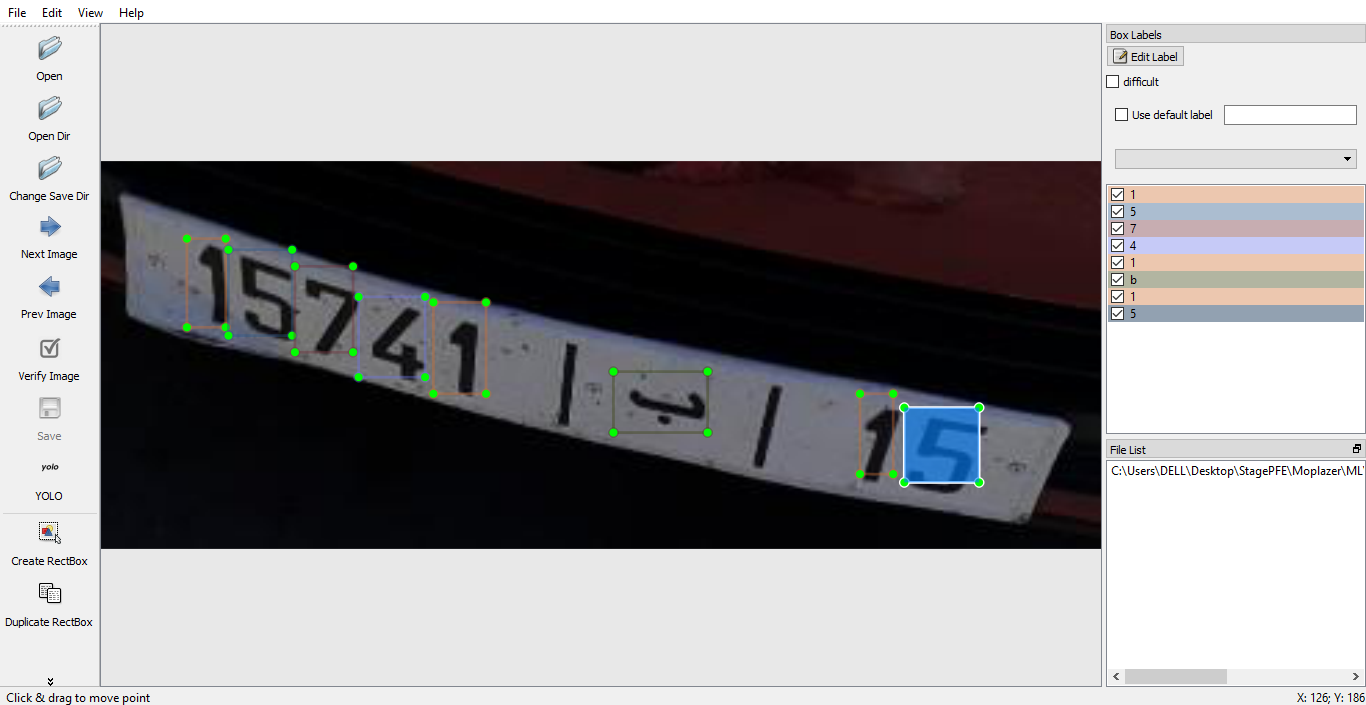
\includegraphics[scale=0.3]{exampleAnnotation}
        \caption{Exemple d'annotation de plaque sur LabelImg}
    \end{figure}
    \subsection{Nettoyage et préparation}
    Pour cette phase, nous avons dans un premier temps effectuer quelques prétraitements sur les images collectées (redimensionnement et auto-orientation). Dans un second temps, pour augmenter le volume des données, nous avons créé de nouvelles données à partir des 3570 originales. Cette augmentation a été faite sur la plateforme Roboflow en utilisant plusieurs procédés comme la \textbf{saturation}, \textbf{modification de la luminosité}, l’\textbf{ajout des bruits et de flous}. Ces procédés nous ont permis d’avoir au total \textbf{8989 images annotées de plaques marocaines}. Nous avons analysé les proportions de chaque classes dans notre base de 8989 images et le graphe suivant les illustre. 
        \begin{figure}[H]
            \centering
            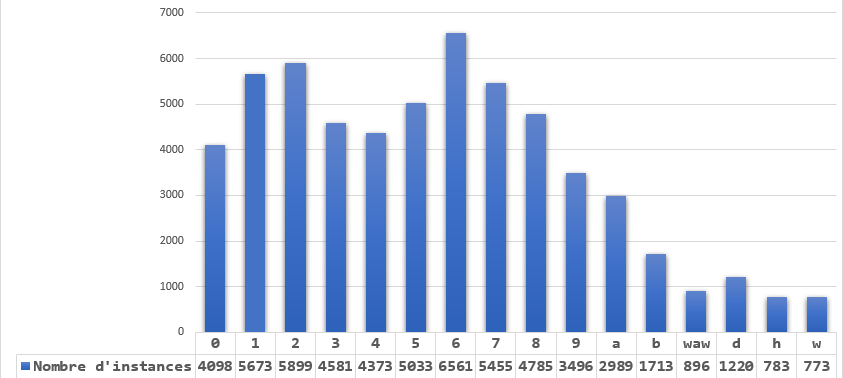
\includegraphics[scale=0.5]{proportionsClasses}
            \caption{Proportions des classes}
        \end{figure}
    \subsection{Entraînement du modèle}
    Avant l’entraînement proprement dit, nous avons subdivisé nos deux données en deux: \textbf{90\% pour l’entraînement et 10\% pour le test}. Nous avons par la suite effectué l’entraînement sur Google Colab avec les mêmes paramètres que précédemment sauf quelques modifications:
    \begin{itemize}
        \item \textbf{Utilisation du \href{https://github.com/AlexeyAB/darknet/}{repertoire darknet d'AlexeyAB}}
        \item \textbf{Utilisation de fichier de configuration} \href{https://github.com/AlexeyAB/darknet/blob/master/cfg/yolov4-tiny-3l.cfg}{yolov4-tiny\_3l.cfg}: toutefois, nous avons modifié certains paramètres dans ce fichier.
        \begin{table}[H]
            \centering
            \begin{tabular}{|l|c|}
                \hline
                \rowcolor{Gray}
                \textbf{Paramètres} & \textbf{Nouvelle valeur} \\ \hline
                batch & \textbf{64} \\ \hline
                subdivisions & \textbf{32} \\ \hline
                width & \textbf{416} \\ \hline
                height & \textbf{416} \\ \hline
                max\_batches & \textbf{10000} \\ \hline
                steps & \textbf{8000, 9000} \\ \hline
                classes & \textbf{16} \\ \hline
                filters (couche de convolution avant couche yolo) & \textbf{63} \\ \hline 
            \end{tabular}
            \caption{Quelques paramètres du fichier de configuration YOLO pour le modèle OCR}
        \end{table}
    \end{itemize}
    Le graphe suivant montre l'évolution de la performance du modèle au cours de l'entraînement: la précision maximale atteinte par le modèle est de \textbf{95,1\%}.
        \begin{figure}[H]
            \centering
            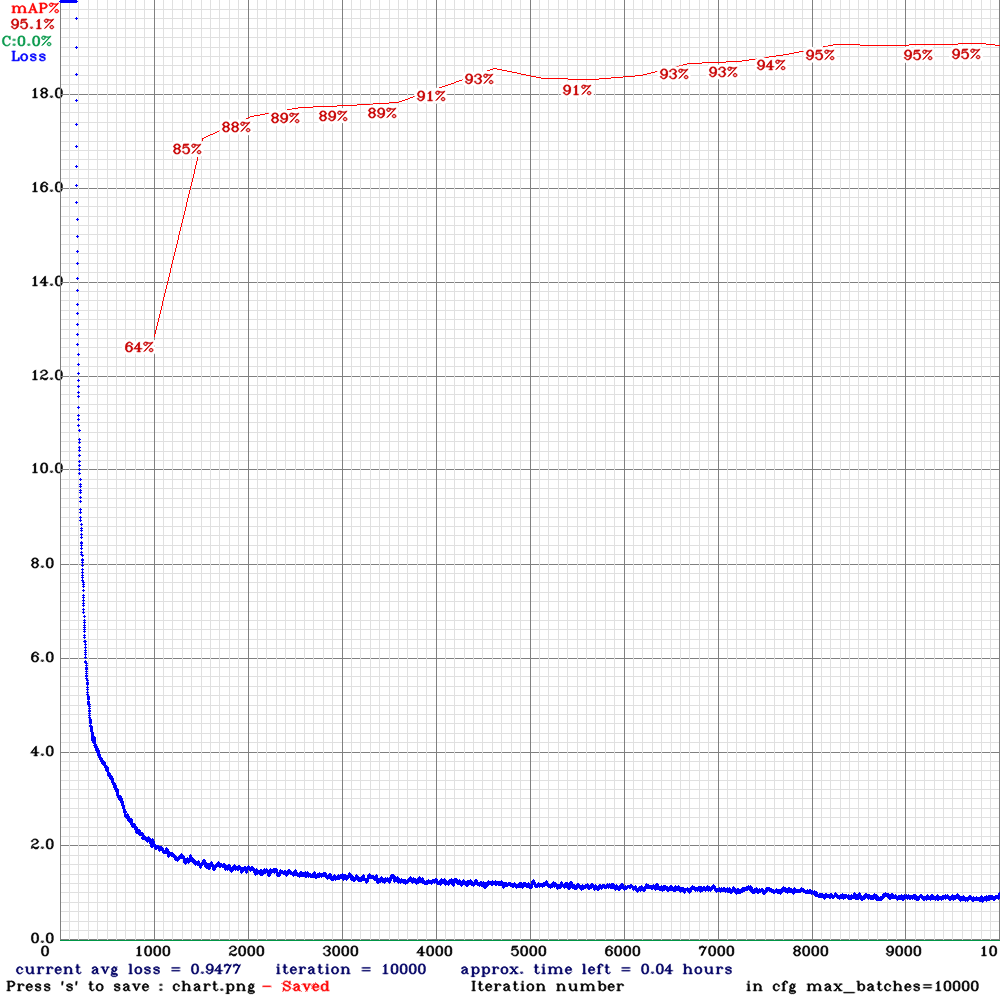
\includegraphics[scale=0.3]{chart2.png}
            \caption{Évolution de la performance du modèle}
        \end{figure}
    \subsection{Résultats et évaluation}
    Pour évaluer notre modèle de lecture du matricule, nous avons collecté des images contenant des véhicules. Dans un premier temps, nous avons utilisé le modèle de détection de plaques pour localiser les plaques sur les images. Dans un second temps, nous avons utilisé le modèle courant pour détecter les caractères sur les plaques. Le tableau suivant les résultats de la performance du modèle.
    \begin{table}[H]
        \centering
        \begin{tabular}{|l|l|}
            \hline
            \rowcolor{Gray}
            \textbf{Évaluation} & \textbf{Valeur} \\ \hline
            Nombre de caractères correctement détectés (VP) & \textbf{302} \\ \hline
            Nombre de caractères non détectés (FN) & \textbf{11} \\ \hline
            Nombre de fausses détections (FP) & \textbf{12} \\ \hline
            Précision & \textbf{96,18\%} \\ \hline
            Rappel & \textbf{96,48\%} \\ \hline
        \end{tabular}
        \caption{Évaluation du modèle de lecture du matricule}
    \end{table}
    Comme pour le modèle de détection de plaques, la précision et le rappel du modèle de lecture des matricules sont très élevés. Ceci nous permet de dire que notre système est globalement très précis. Voici quelques exemples de lecture des plaques d'immatriculation.
    \begin{figure}[H]
        \begin{subfigure}{0.3\textwidth}
            \centering
            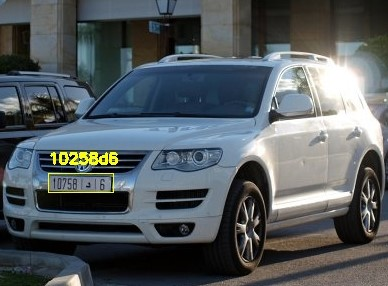
\includegraphics[width=\textwidth]{plateDetect1}
        \end{subfigure}
        \hfill
        \begin{subfigure}{0.3\textwidth}
            \centering
            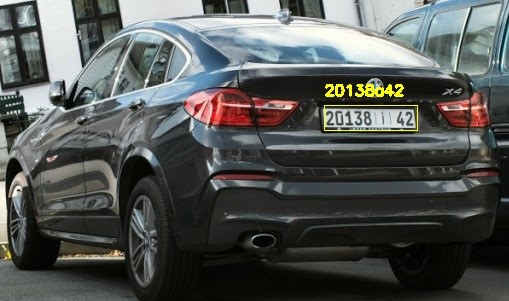
\includegraphics[width=\textwidth]{plateDetect2}
        \end{subfigure}
        \hfill
        \begin{subfigure}{0.3\textwidth}
            \centering
            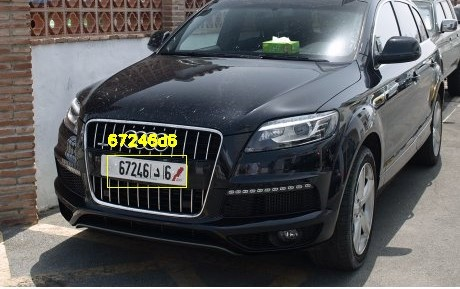
\includegraphics[width=\textwidth]{plateDetect3}
        \end{subfigure}
        \caption{Exemples de lecture des matricules des véhicules}
    \end{figure}


    \section{Conclusion}
    Nous arrivons au terme d’un des chapitres les plus importants de notre document. Il  nous a permis de présenter en détail notre système de reconnaissance des plaques d’immatriculation marocaines. Nous pouvons retenir que notre système ANPR que nous avons choisi d’appeler MoPlaZer est constitué de deux parties essentielles. La première partie est consacrée à la détection de la plaque d’immatriculation sur une image. Nous avons vu que pour arriver à détecter les plaques, nous avons entraîné un modèle de détection d’objets avec YOLOv4. La précision de ce modèle est de 99,7\%. La seconde partie de notre système est dédiée à la lecture du matricule: extraire en format textuel le numéro d’immatriculation. Pour y arriver, nous avons aussi entraîné un modèle de détection d’objets avec YOLOv4. Ce modèle atteint une précision de plus de 96\%. Nous pouvons donc constater que notre système MoPlaZer est globalement précis. Après avoir conçu et réalisé le système, il faut l’intégrer dans des cas d’utilisation particulière. C’est l’objet du prochain et dernier chapitre.
